\begin{frame}[fragile]{Non-Linear Kernel}
  Dual form of the primary Lagrangian problem:
  \newline
  \begin{equation*}
    \begin{split}
      \textcolor{blue}{\max_{\alpha}}\ &\ \textcolor{blue}{L_D}\ 
      \equiv\ 
      \textcolor{lightgray}{\sum_{i=1}^{L} \alpha_i - \frac{1}{2} \alpha^T} 
      \mathbf{\textcolor{blue}{H}}
      \textcolor{lightgray}{\alpha}
    \end{split}
  \end{equation*}

  where:
  \newline
  \begin{equation*}
    \textcolor{blue}{H}\ \equiv\ \textcolor{lightgray}{y_i y_j} \mathbf{\textcolor{blue}{k(x_i, x_j)}}
  \end{equation*}

  linear kernel is defined as:
  \begin{equation*}
    k(x_i, x_j) = \phi(x_i) \cdot \phi(x_j)
  \end{equation*}

  polynomial kernel is defined as:
  \begin{equation*}
    k(x_i, x_j) = (\phi(x_i) \cdot \phi(x_j) + 1)^{deg}
  \end{equation*}
\end{frame}

\begin{frame}[fragile]{Non-Linear Kernel}
  \begin{columns}[onlytextwidth, T, c]
    \begin{column}{.5\textwidth}
        \begin{figure}
            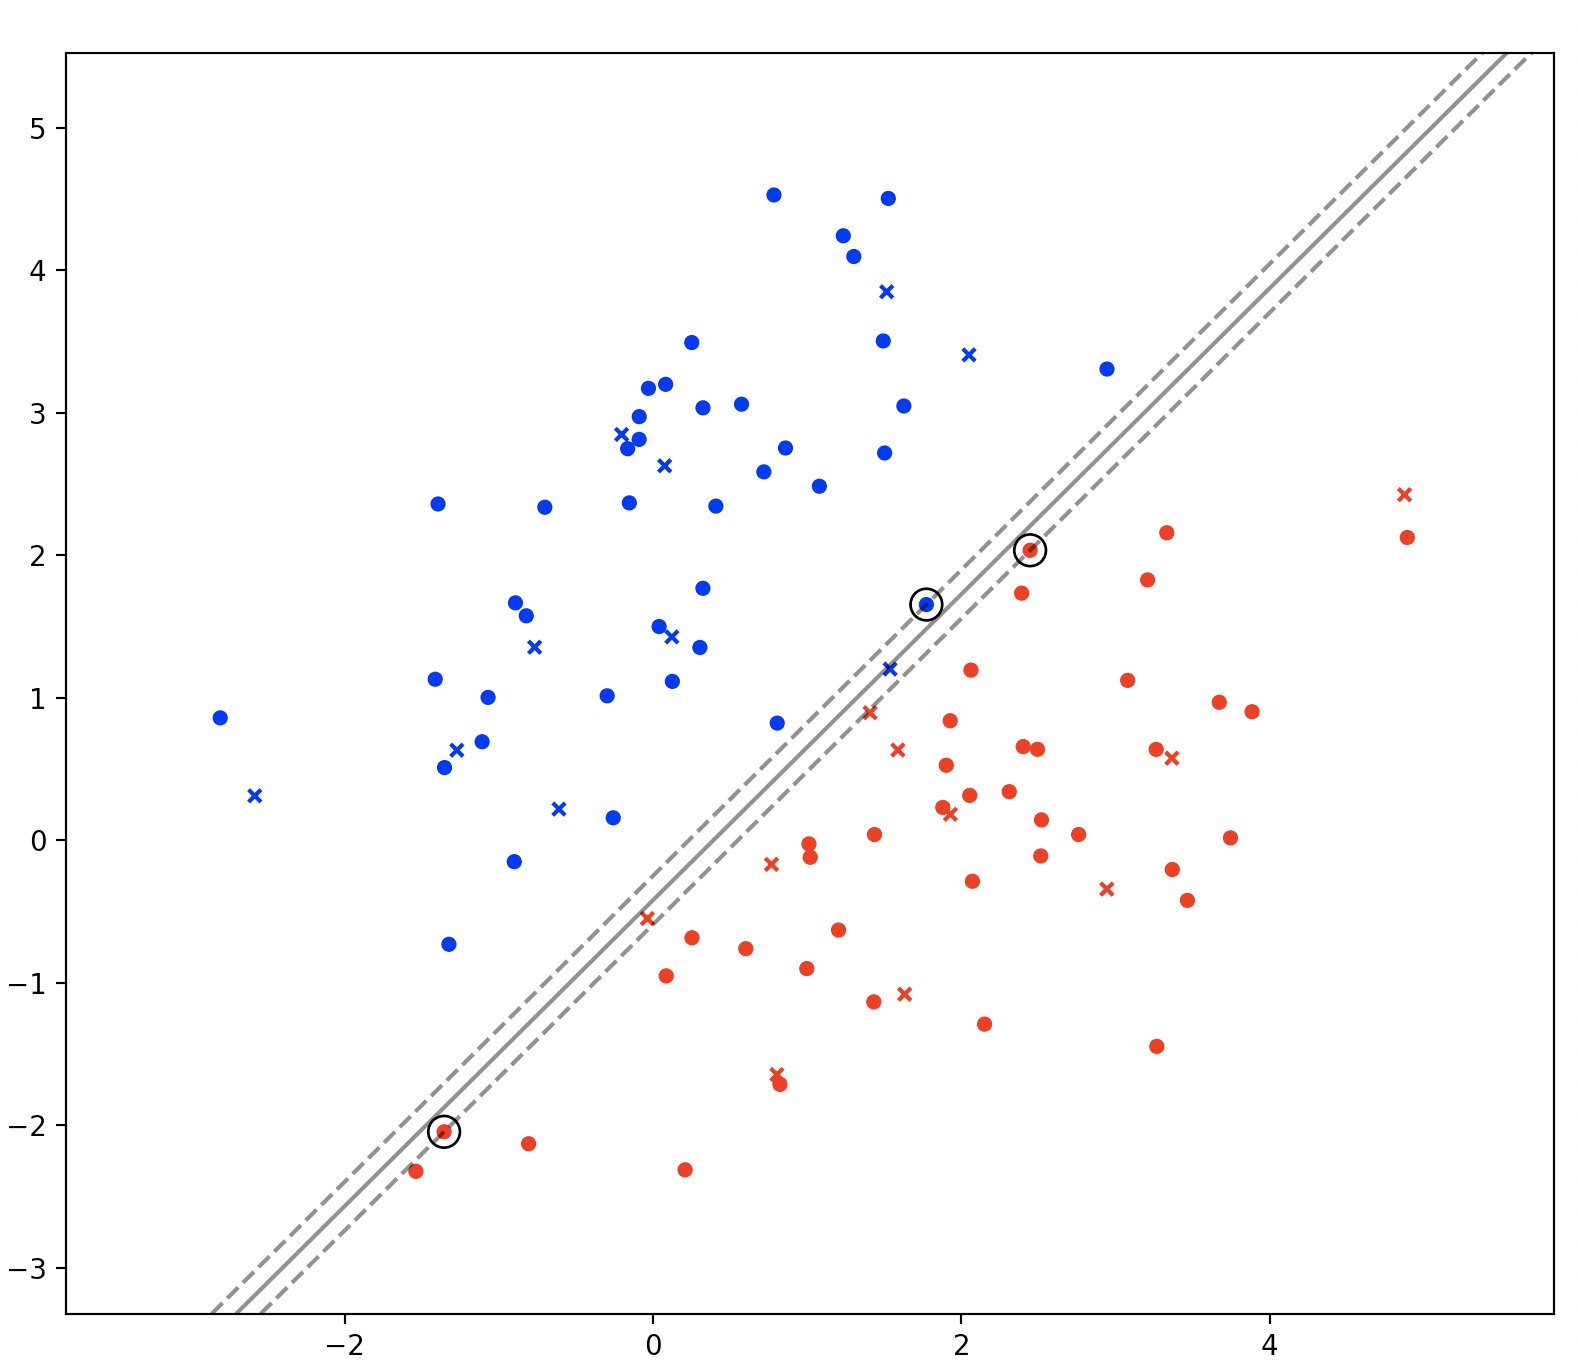
\includegraphics[width=5cm]{assets/images/s4.01.png}
            \caption{Linear Kernel}
        \end{figure}
    \end{column}
    \begin{column}{.5\textwidth}
        \begin{figure}
            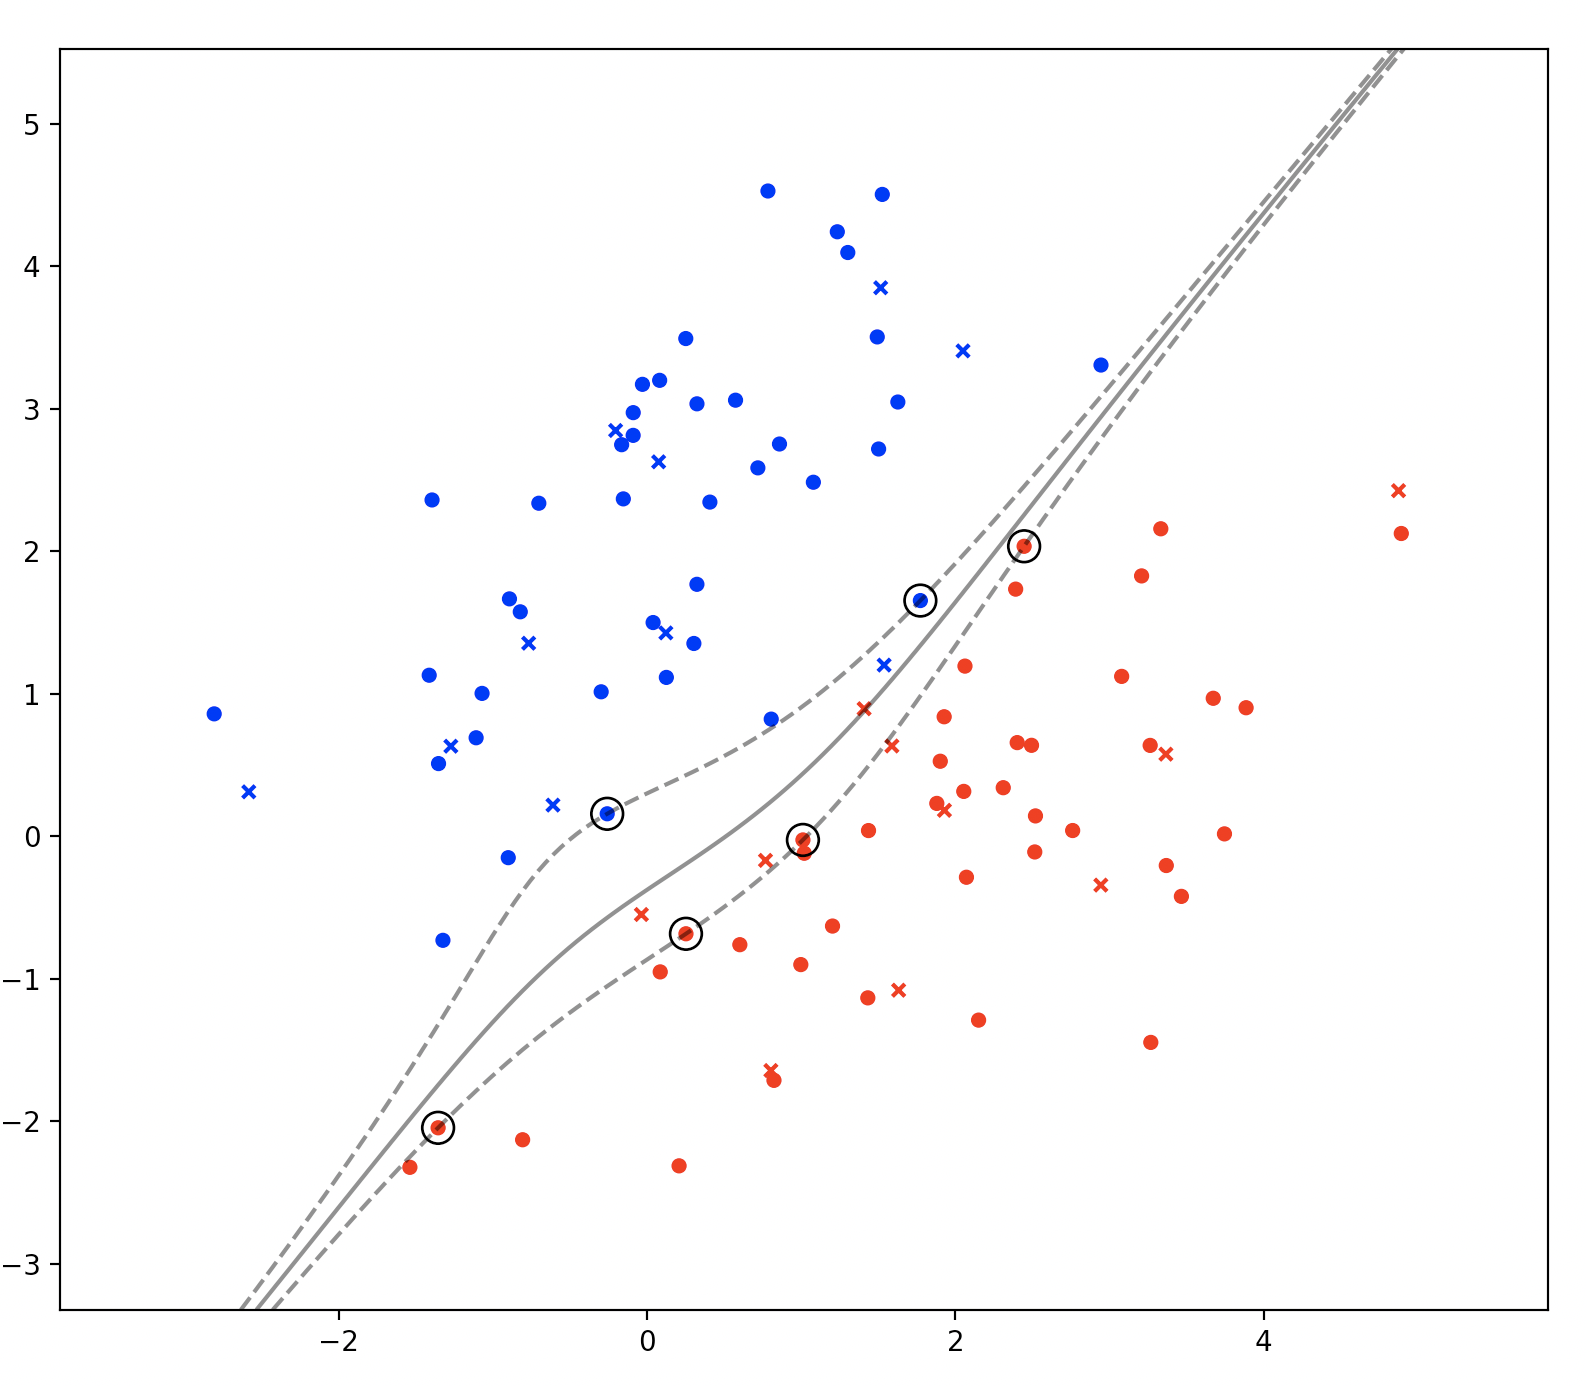
\includegraphics[width=5cm]{assets/images/s4.02.png}
            \caption{Polynomial Kernel}
        \end{figure}
    \end{column}    
  \end{columns}
\end{frame}
